\RequirePackage{luatex85}
\documentclass[border=6pt]{standalone}
\usepackage{tikz}
\usepackage[compat=1.1.0]{tikz-feynman}
\usepackage{amsmath}
\usetikzlibrary{decorations.pathmorphing,decorations.markings,arrows.meta,patterns}

\begin{document}
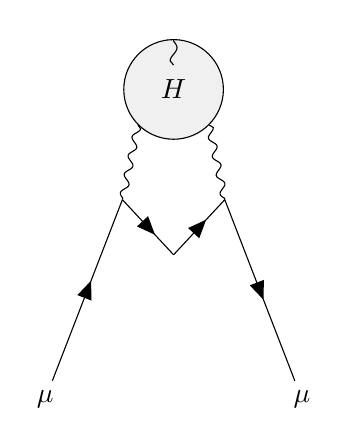
\begin{tikzpicture}
\begin{feynman}
  \vertex (top) {\(\times\)};
  \vertex [circle, draw, fill=gray!12, minimum size=36pt, inner sep=0pt, below=0.55cm of top] (H) {\(H\)};
  \vertex [below=2.1cm of H] (vtx);
  \vertex [below left=1.6cm and 1.4cm of vtx] (lmu) {\(\mu\)};
  \vertex [below right=1.6cm and 1.4cm of vtx] (rmu) {\(\mu\)};
  \vertex [above left=0.7cm and 0.65cm of vtx] (lconn);
  \vertex [above right=0.7cm and 0.65cm of vtx] (rconn);
  \diagram* {
    (lmu) -- [fermion] (lconn) -- [fermion] (vtx) -- [fermion] (rconn) -- [fermion] (rmu),
    (H) -- [photon] (top),
    (lconn) -- [photon] (H.south west),
    (rconn) -- [photon] (H.south east),
  };
\end{feynman}
\end{tikzpicture}
\end{document}
